\begin{blocksection}
\question
Construct an FSM that outputs ones until 3 consecutive zeroes have appeared, at which point it outputs zeroes. How many states do we need?

\begin{solution}[1.5in]
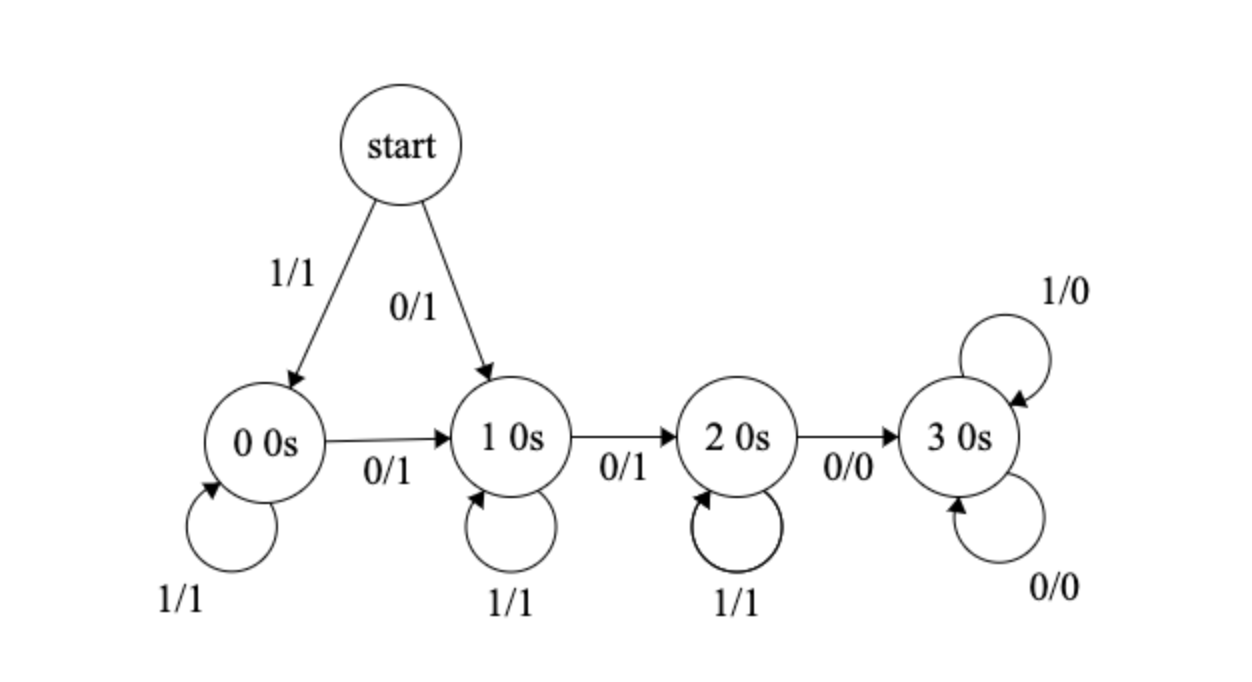
\includegraphics[width=\textwidth]{midterm2/fsm1}
We will need 4 states (without a START state) or 5 states (with a START state).
\end{solution}

\question
How many states would we need to construct an FSM that outputs ones until $n$ non-consecutive zeroes have appeared?

\begin{solution}[0.7in]
Either $n + 1$ without a start state or $n + 2$ with a start state.
\end{solution}

\question
Construct an FSM that returns the XOR of all the inputs.

\begin{solution}[0.7in]
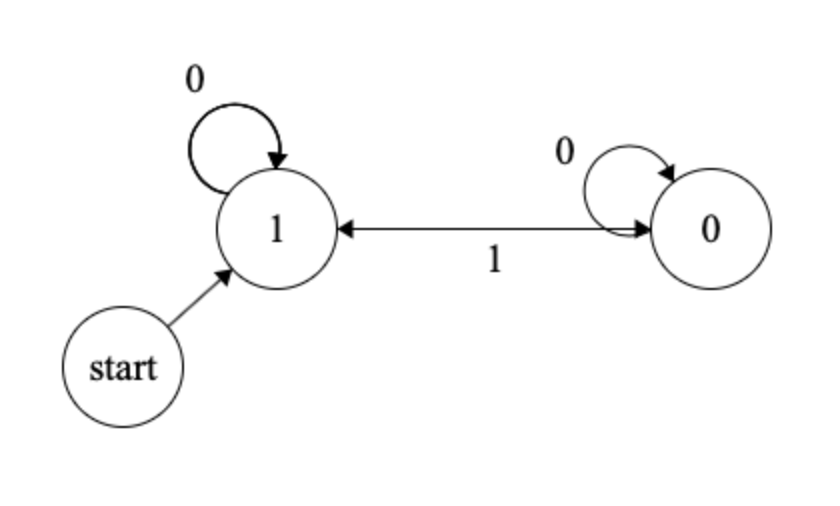
\includegraphics[width=\textwidth]{midterm2/fsm2}
The values in the nodes are the outputs of the states.
\end{solution}

\end{blocksection}